%\documentclass[12pt,a4paper,openright,twoside]{report}
\documentclass{standalone}
\usepackage{fancyhdr}
\usepackage{indentfirst}
\usepackage{graphicx}
\usepackage{newlfont}
\usepackage{amssymb}
\usepackage{amsmath}
\usepackage{latexsym}
\usepackage{amsthm}
\usepackage{enumitem}
\usepackage{subfig}
\usepackage[hidelinks]{hyperref}
\usepackage{float}
\usepackage{siunitx}

\usepackage{color}
\usepackage{eurosym}
\usepackage{subfloat}
\usepackage{subcaption}

%\usepackage{ucs}
%\usepackage[italian]{babel}
%\usepackage[T1]{fontenc}
%\usepackage[latin1]{inputenc}


%\oddsidemargin=30pt \evensidemargin=20pt%impostano i margini
%\hyphenation{sil-la-ba-zio-ne pa-ren-te-si}%serve per la sillabazione: tra parentesi

%\pagestyle{fancy}\addtolength{\headwidth}{20pt}
%\renewcommand{\chaptermark}[1]{\markboth{\thechapter.\ #1}{}}
%\renewcommand{\sectionmark}[1]{\markright{\thesection \ #1}{}}
%\rhead[\fancyplain{}{\bfseries\leftmark}]{\fancyplain{}{\bfseries\thepage}}
%\cfoot{}
%%%%%%%%%%%%%%%%%%%%%%%%%%%%%%%%%%%%%%%%%
%\linespread{1.3}                        %comando per impostare l'interlinea
%
\begin{document}
	
	\chapter{Misure Preliminari}                %crea il capitolo
	%%%%%%%%%%%%%%%%%%%%%%%%%%%%%%%%%%%%%%%%%imposta l'intestazione di pagina
	%\lhead[\fancyplain{}{\bfseries\thepage}]{\fancyplain{}{\bfseries\rightmark}}
	%\pagenumbering{arabic}
	
	
	
	\section{Misura della tensione di lavoro}
	\label{sec:tension}                %crea la sezione
	Per la prima delle misure preliminari abbiamo dovuto stimare la tensione di lavoro ideale per due dei fotomoltiplicatori impiegati dal telescopio. Se viene applicata infatti una tensione troppo bassa la valanga degli elettroni non viene prodotta affatto, mentre se questa \`e troppo elevata si va a generare una corrente di buio dovuta agli $e^-$ termici sul fotocatodo che producono un segnale in assenza di una particella passante e possono portare a saturazione danneggiando il dispositivo.\\
	Nello specifico si \`e deciso di utilizzare i PM R00B e L00B, ovvero due fotomoltiplicatori posti ai capi del medesimo scintillatore. Questa \`e infatti sembrata la scelta pi\`u opportuna se si pensa che per ottenere la tensione di lavoro dei due sensori, si sono studiati il numero di rivelazioni coincidenti  di muoni cosmici passanti (uniche particelle presenti nei raggi cosmici, se si escludono i neutrini che non producono segnale, che sono in grado di superare la lastra di ferro intatti). Solo nel caso in cui i due PM appartengano allo stesso scintillatore si pu\`o essere fiduciosi del fatto che i due segnali in coincidenza siano dovuti al passaggio della stessa particella; se si fossero scelti due PM appartenenti allo stesso piano ma a scintillatori diversi, si sarebbe avuta la certezza di avere solo coincidenze accidentali, mentre nel caso li si fosse presi in due piani separati si sarebbe corso il rischio di perdere tutte le coincidenze dovute a muoni passanti con una sufficiente inclinazione verticale, oltre a rischiare coincidenze accidentali dovute a due muoni vicini passanti singolarmente sui due rivelatori.\\
	Per procedere con la misura si \`e lasciata costante la tensione applicata a uno dei fotomoltiplicatori variando progressivamente quella dell'altro e si sono misurati il numero di segnali in coincidenza per ogni valore, ottenendo una curva come quella in Figura \ref{fig:curva-tens}. Si \`e quindi fissata la stima della tensione ottenuta per il primo PM e si \`e ripetuto il processo variando quella del secondo. L'andamento delle curve \`e in un primo momento crescente quando ancora la tensione \`e troppo bassa e la moltiplicazione a valanga non avviene a pieno regime, seguito da un plateau in cui entrambi i PM lavorano correttamente e infine una salita vertiginosa dovuta al regime di scarica, che si \`e per\`o cercato di eludere in modo da non danneggiare gli apparati. I valori stimati sono stati ottenuti scegliendo le tensioni corrispondenti a met\`a del plateau e sono tabulati in Tabella \ref{tab:tension}.\\
	
	\begin{table}[h]                        %ambiente tabella
		%(serve per avere la legenda)
		\begin{center}                          %centra nella pagina la tabella
			\begin{tabular}{r|c|c}                  %tre colonne con righe verticali
				%   prodotte con |
				\hline \hline                           %inserisce due righe orizzontali
				PM & $Tensione\ di \ lavoro$\\           %& separa le colonne e con
				\hline                                  %inserisce una riga orizzontale
				L00B & $825\ mV$ \\           %  \\ va a capo
				\hline                                  %inserisce una riga orizzontale
				R00B & $850\ mV$ \\
				\hline \hline                           %inserisce due righe orizzontali
			\end{tabular}
			\caption{tabella contenente le tensioni di lavoro stimate per i PM}
			\label{tab:tension}
		\end{center}
	\end{table}
	
	\begin{figure}[H]
		\begin{center}
			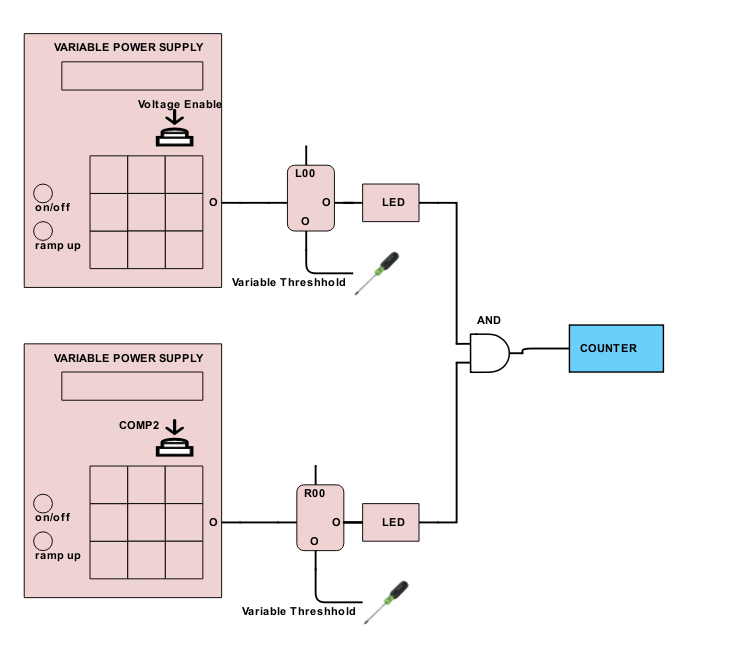
\includegraphics[width=0.78\textwidth]{./SCHEMI/Tension.png} % Include the image placeholder.png
			\caption{\small Rappresentazione schematica del circuito utilizzato per la calibrazione della tensione di lavoro e delle soglie di discriminazione dei fotomoltiplicatori}
			\label{fig:circ-tens}
		\end{center}
	\end{figure}
	
	\begin{figure}[H]
		\begin{center}
			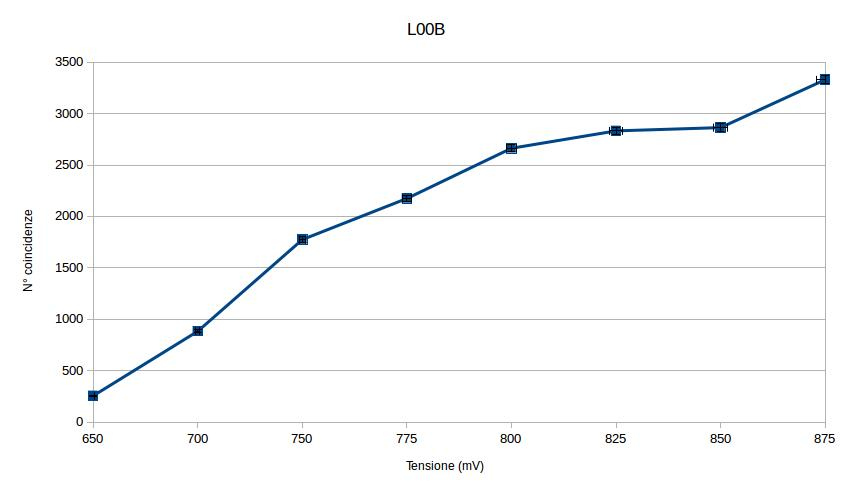
\includegraphics[width=1\textwidth]{./excel-plots/tension-L00c.jpg} % Include the image placeholder.png
			\bigbreak
			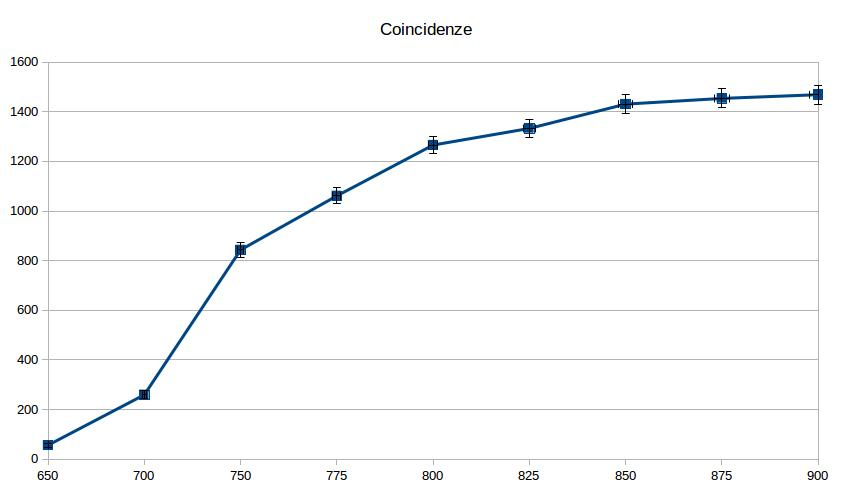
\includegraphics[width=1\textwidth]{./excel-plots/tension-R00c.jpg} % Include the image placeholder.png
			\caption{\small Curve di calibrazione della tensione data dal numero di coincidenze di segnale tra i PM L00B e R00B al variare della tensione applicata al secondo, con quella del primo lasciata costante (in basso) e viceversa (in alto)}
			\label{fig:curva-tens}
		\end{center}
	\end{figure}
	\clearpage
	Il circuito realizzato per eseguire le misure \`e invece schematizzato in Figura \ref{fig:circ-tens} e consiste di due generatori di tensione variabili (CAEN Mod.470) che alimentano i due PM. Il segnale analogico prodotto da questi viene quindi fatto passare attraverso dei discriminatori LED (CAEN Mod.840) che lo trasformano in un segnale digitale standard NIM costituito da un impulso di onda quadra larga 40ns e profonda -800 mV. I segnali digitalizzati dei due PM sono quindi portati in coincidenza tramite un modulo logico AND (CAEN Mod 405),collegato a sua volta un modulo counter, con il quale \`e  stato possibile contare il numero totale di corrispondenze per un tempo di presa dati impostato a 90s. Sebbene non sia rappresentato in figura, i conteggi sono stati effettuati in maniera analoga anche  per i singoli canali, che sono stati sdoppiati utilizzando dei moduli FAN I/O, e collegati individualmente a degli ulteriori moduli counter.\\
	
	
	\section{Curve di ritardo}
	\label{sec:delay}
	Il trigger definitivo usato per la misura della vita media del muone (vedi Sezione \ref{sec:trigger}) richiede l'utilizzo di scintillatori su semipiani successivi che vadano a misurare dei segnali in coincidenza dovuti al passaggio della medesima particella.\\
	Per ottenere un segnale di coincidenza si sono dovuti prima digitalizzare i due segnali analogici tramite l'uso di discriminatori, e poi sfruttare un modulo logico che fornisca un segnale in uscita solo sei i due input si sovrappongono per una certa finestra temporale. E' evidente che i segnali prodotti su due piani di scintillatori successivi non sono mai perfettamente contemporanei, in quanto la particella passante impiega una certa quantit\`a di tempo a percorrere la distanza che li separa. \\
	Risulta necessario, quindi, conoscere con una certa precisione quale sia il ritardo massimo oltre il quale due segnali in coincidenza non vengono pi\`u interpretati come tali. Ci si aspetta che questo risulti approssimativamente pari alla larghezza dell'onda quadra di un segnale NIM, che corrisponde a 40 ns.\\
	Per effettuare tale stima, si considerano due  PM corrispondenti a due semipiani successivi, e si rivelano i muoni passanti ritardando il segnale di uno e lasciando intatto quello dell'altro e viceversa. Introducendo ritardi via via pi\`u grandi e misurando il numero di coincidenze osservate si ottengono quindi quelle che vengono definite curve di ritardo. Nello specifico in Figura \ref{fig:delay} si possono osservare quelle ottenute per i PM R00B e R10B.\\
	Idealmente tali curve dovrebbero avere una forma a gradino con il drop in corrispondenza del valore di ritardo massimo oltre il quale si perdono le coincidenze. In realt\`a l'andamento \`e decisamente meno netto a causa di effetti introdotti dall'elettronica, quali il time-walk (Variazioni nella formazione del segnale digitale dovuti a differenze nelle ampiezze dei segnali analogici)  e il jitter (modifiche nella forma della curva di segnale nel discriminatore a causa del rumore). E' comunque possibile ottenere delle stime per i massimi valori di ritardo, che risultano compatibili col valore atteso di 40 ns e sono state riportate in Tabella \ref{tab:delay}.
	
	\begin{table}[h]                        %ambiente tabella
		%(serve per avere la legenda)
		\begin{center}                          %centra nella pagina la tabella
			\begin{tabular}{r|c|c}                  %tre colonne con righe verticali
				%   prodotte con |
				\hline \hline                           %inserisce due righe orizzontali
				PM & $Ritardi\ massimi$\\           %& separa le colonne e con
				\hline                                  %inserisce una riga orizzontale
				R00 & $40\ ns$ \\           %  \\ va a capo
				\hline                                  %inserisce una riga orizzontale
				R10 & $30\ ns$ \\
				\hline \hline                           %inserisce due righe orizzontali
			\end{tabular}
			\caption{tabella contenente le tensioni di lavoro stimate per i PM}
			\label{tab:delay}
		\end{center}
	\end{table}
	
	
	Si pu\`o osservare  inoltre che le due curve risultano asimmetriche. Questo avviene per via del fatto che il tempo di volo della particella introduce un fattore di ritardo asimmetrico sui due rivelatori: sul piano 1 lo aumenta, laddove sul piano 0 lo diminuisce. E' possibile sfruttare tale effetto per ottenere una stima del tempo di volo effettuando una semplice differenza tra la lunghezza dei due gradini:
	\begin{equation}
	t_{flight}=\Delta t_1-\Delta t_2
	\end{equation}
	Considerando i valori sperimentali ottenuti:
	\begin{equation}
	t_{flight} \sim (40-30)ns=10ns
	\end{equation}
	Si noti infine che le due curve non raggiungono mai lo 0 a causa delle coincidenze introdotte dal rumore.
	\begin{figure}[H]
		\begin{center}
			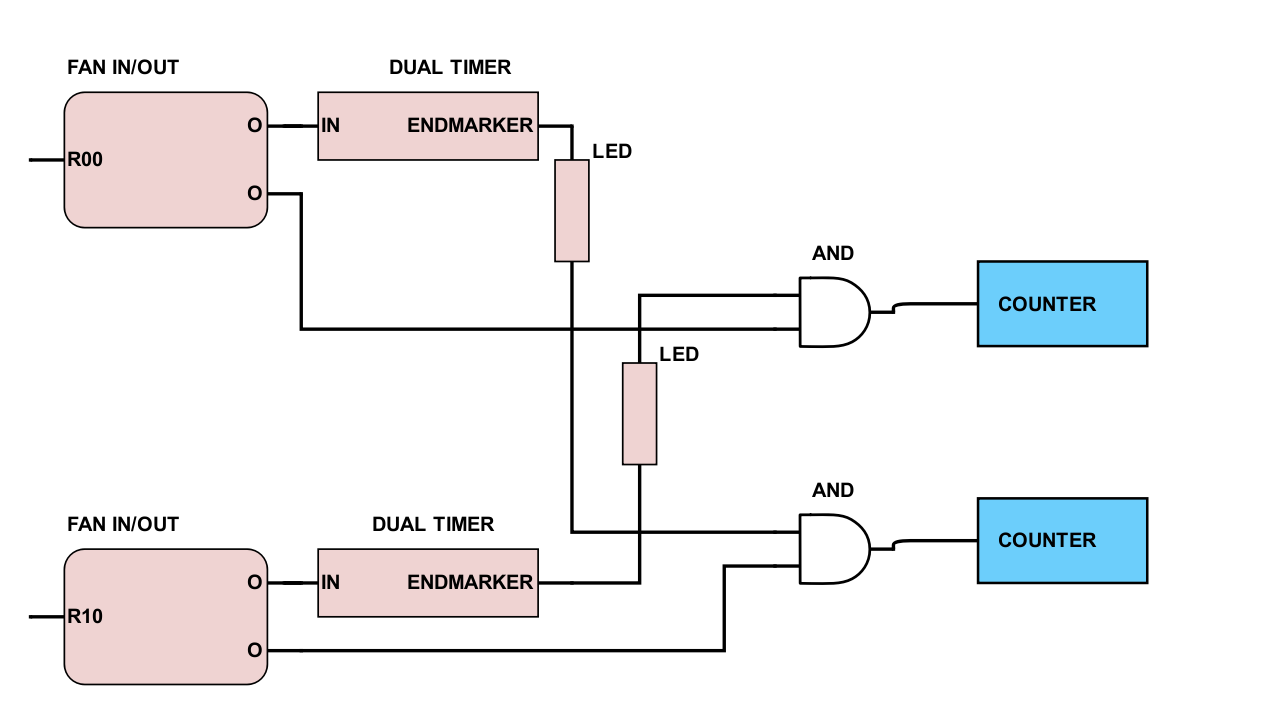
\includegraphics[width=1.2\textwidth]{./SCHEMI/RITARDO.png} % Include the image placeholder.png
			\caption{\small Rappresentazione schematica del circuito utilizzato per determinafre le curve di ritardo per i PM  R00B e R10B}
			\label{fig:circ-delay}
		\end{center}
	\end{figure}
	\begin{figure}[h]
		
		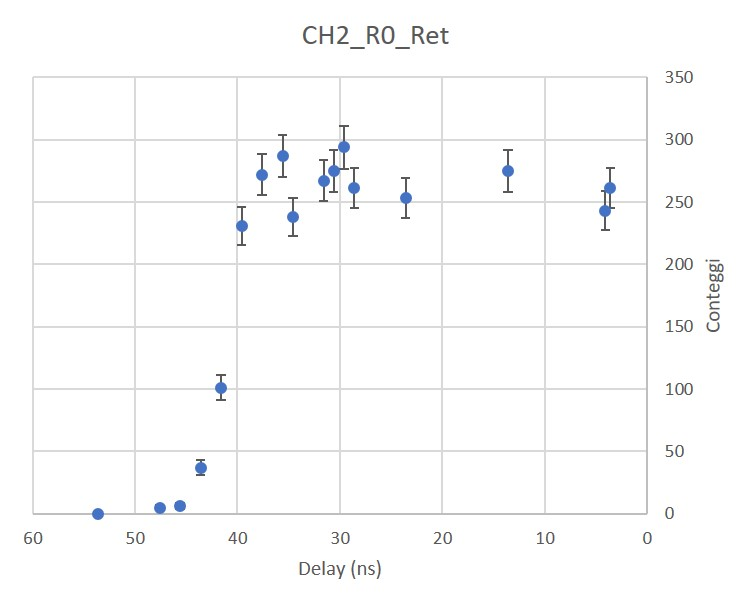
\includegraphics[width=.5\textwidth]{excel-plots/R00-delay-flipped.jpg}\quad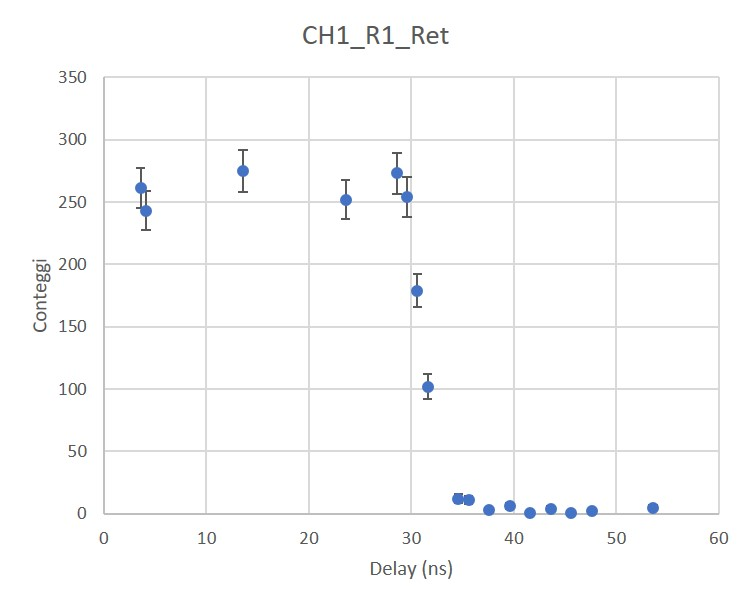
\includegraphics[width=.5\textwidth]{excel-plots/R01-delay.jpg}
		\caption{Curve di ritardo relative ai PM R00 (sinistra) e R10 (destra)}
		\label{fig:delay}
	\end{figure}
	
	
	
	\clearpage
	In Figura \ref{fig:circ-delay} si \`e riportato lo schema corrispondente al circuito utilizzato in questa sezione. Come si pu\`o osservare si \`e fatto uso di due discriminatori per la digitalizzazione del segnale, oltre che di due moduli Dual Timer che permettono di introdurre dei ritardi variabili. Per il conteggio delle coincidenze si sono infine utilizzati due moduli logici in modalit\`a AND e due contatori impostati per 60 s di presa dati. Si pu\`o notare che a causa dell'asimmetria dovuta all'utilizzo del Dual Timer su uno solo dei due percorsi, viene introdotto un ritardo irriducibile che pu\`o essere stimato:
	\begin{equation}
	\Delta t_{irriducibile}=\Delta t_{Cavo}+\Delta t_{Dual\ Timer}=2ns+(1.6\pm 0.5)ns
	\end{equation}
	Dove $\Delta t_{Cavo}$ e $\Delta t_{Dual\ Timer}$  sono rispettivamente i delay introdotti dal cavo di collegamento col Dual Timer e  dall'elettronica interna del modulo stesso. Per entrambi si sono utilizzati i valori nominali.
	
	\section{Curve di discriminazione}
	\label{sec:discrimination}
	Come gi\`a accennato nei precedenti paragrafi, per trasformare i segnali analogici forniti dai fotomoltiplicatori in segnali digitali standard NIM si \`e fatto uso di moduli chiamati discriminatori. Questi dispositivi ricevono un segnale di tensione in input e ne restituiscono uno in output solo se il segnale supera una soglia di tensione negativa. Il threshold di tali dispositivi \`e impostabile e deve essere scelto con cura; infatti se questo \`e troppo elevato in valore assoluto si rischia di rigettare degli eventi di segnale, laddove se \`e troppo basso il rumore non viene eliminato correttamente.\\
	Per selezionare la soglia di discriminazione corretta per ognuna delle triplette di PM si \`e adottato un procedimento del tutto analogo a quello descritto nella Sezione \ref{sec:tension}: si \`e lasciato intatto il threshold di una tripletta di PM (-40mV), andando a variare in maniera progressiva quella di un altro e si \`e quindi usato un contatore per misurare il numero di coincidenze ottenute per ogni valore in un certo intervallo di tempo.\\
	La curva che si ottiene \`e detta di discriminazione e presenta una discesa ripida (gli eventi diminuiscono man mano che si elimina il rumore), seguita da un plateau e infine da un' ulteriore discesa (oltre un certo valore gli eventi di segnale incominciano a essere scartati). Se ne riporta quella relativa al PM R00 in Figura \ref{fig:discrimination}, mentre tutte le altre sono lasciate in Appendice.\\
	
	\begin{figure}[H]
		\begin{center}
			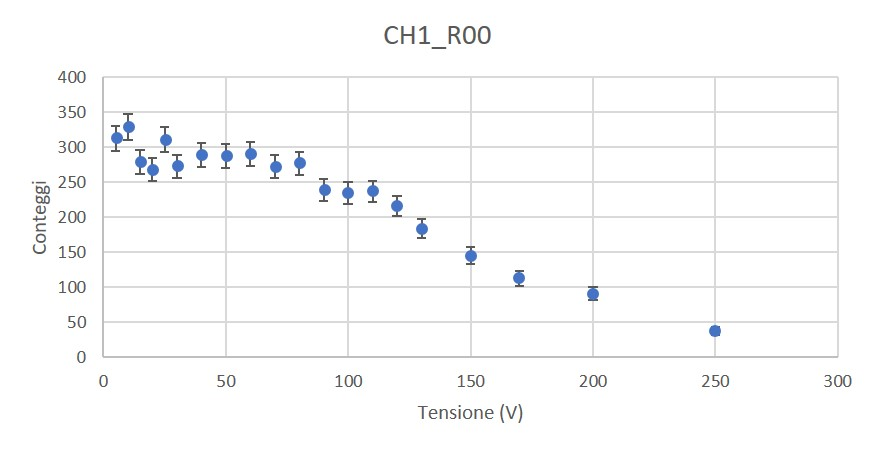
\includegraphics[width=1\textwidth]{./excel-plots/disc-R00.jpg} % Include the image placeholder.png
			\caption{\small Curva di discriminazione relativa al PM R00, collegato al canale 1 dei moduli logici AND}
			\label{fig:discrimination}
		\end{center}
	\end{figure}
	
	I theshold sono stati selezionati andando a misurare il valore medio del plateau e sono riportati in Tabella \ref{tab:discrimination}.
	\begin{table}[H]                        %ambiente tabella
		%(serve per avere la legenda)
		\begin{center}                          %centra nella pagina la tabella
			\begin{tabular}{r|c|c|c}                  %tre colonne con righe verticali
				%   prodotte con |
				\hline \hline                           %inserisce due righe orizzontali
				PM & Soglia (mV) & PM & Soglia (mV) \\           %& separa le colonne e con
				\hline                                  %inserisce una riga orizzontale
				$L00$ & $-65$ & $R00$ & -48 \\           %  \\ va a capo
				\hline                                  %inserisce una riga orizzontale
				$L10$ & $-73$ & $R10$ & -65 \\           %  \\ va a capo
				\hline       
				$L01$ & $-20$ & $R01$ & -65 \\           %  \\ va a capo
				\hline       
				$L11$ & $-80$ & $R11$ & -20 \\           %  \\ va a capo
				
				\hline \hline                           %inserisce due righe orizzontali
			\end{tabular}
			\caption{Tabella contenente i valori stimati dei threshold}
			\label{tab:discrimination}
		\end{center}
	\end{table}
	
	Il circuito utilizzato \`e concettualmente identico a quello in Figura \ref{fig:circ-delay}, con la sola aggiunta di svariati canali di FAN I/O che hanno permesso di effettuare le operazioni su tutti i PM in parallelo.
	
	
	
	
	
	%%%%%%%%%%%%%%%%%%%%%%%%%%%%%%%%%%%%%%%%%%%%%%%%%%%%%%%%%%%%%%%%%%%%%%%%%%%%%%%%%%%%%%%%%%%%%%%%%%%%%%%%%%%%%%%%%%%%%%%%%%%%%%%%%%%%%%%%%%%%%%%%%%%%%%
	
	
	\chapter{Misura della vita media del Muone}
	Per poter misurare la vita media dei muoni provenienti dai raggi cosmici \`e necessario costruire un circuito di trigger che permetta di selezionare eventi di tipo $\mu$-stop, ovvero tali per cui le particelle $\mu$ si fermano nella lastra di ferro presente tra i piani 1 e 2 del rivelatore. Questo segnale funger\`a da start per un modulo TDC (time to digital converter), che grazie al suo clock interno incomincer\`a a misurare il tempo trascorso fino all'arrivo di un segnale di stop rappresentato dal passaggio di un elettrone di decadimento su uno qualsiasi degli scintillatori.
\section{Il Trigger}
\label{sec:trigger}
Come gi\`a accennato, il trigger che vogliamo creare deve essere in grado di selezionare eventi di tipo $\mu$-stop in cui il muone passa attraverso i primi due piani di scintillazione, per poi fermarsi nella sottile lastra di ferro tra il piano 1 e 2, dove infine decade. Questo significa che vorremo una coincidenza di segnale tra il piano 0 e il piano 1 e un'assenza sul piano 2.\\
 In termini di funzioni logiche tale richiesta si pu\`o tradurre come:
\begin{equation}
\begin{split}
T=P_0 \land P_1 \land \overline{P_2}
\\
con\\
P_0=[(L00\land R00)\lor (L01\land R01)]\\
P_1=[(L10\land R10)\lor (L11\land R11)]\\
P_2=[(L20\land R20)\lor (L21\land R21)]
\end{split}
\end{equation}
\\
Il circuito equivalente \`e riportato in Figura \ref{fig:circ-trigger}.

\begin{figure}[H]
	\begin{center}
		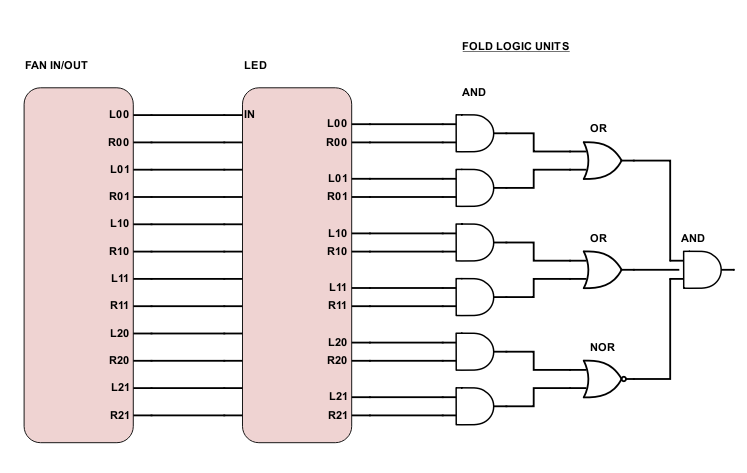
\includegraphics[width=1\textwidth]{./SCHEMI/TriggerMu.png} % Include the image placeholder.png
		\caption{\small Rappresentazione schematica del circuito di trigger di $\mu$-stop}
		\label{fig:circ-trigger}
	\end{center}
\end{figure}
\clearpage
\section{Calibrazione dei TDC}
Il TDC (Time to Digital Converter ) \`e un modulo di elettronica CAMAC (Computer Automated Measurement And Control ) che permette di misurare intervalli temporali. Esso \`e dotato di un common start che fa partire il suo cronometro interno e di 8 canali di stop che interrompono il conteggio. Essendo un modulo CAMAC il TDC pu\`o quindi essere associato a un opportuno software che converta i conteggi del clock in misure di tempo.
\\
I tempi misurati dalla TDC sono in unit\`a standard (stringhe di dati a 12 bit), che devono poi essere tradotte in secondi tramite una costante di conversione. Essa \`e riportata dal costruttore per ogni canale, ma pu\`o variare col tempo e l'usura. E' quindi opportuno trovare le costanti attuali misurando degli intervalli temporali noti tramite i moduli TDC, producendo una retta di calibrazione (I grafici sono lasciati in Appendice). Eseguendo quindi un fit di tali rette sar\`a possibile avere una stima dei fattori :
\begin{equation}
y=a+bt
\end{equation}
Dove $y$ \`e il tempo misurato in arbitrary units, $t$ \`e il valore noto in secondi, $a$ \`e il valore di off-set e $b$ \`e il fattore di conversione.
\\
Gli intervalli di tempo dal valore noto possono essere ottenuti sfruttando il segnale artificiale  di un modulo Dual Timer (vedi Figura \ref{fig:circ-calibrazione}), fissato tramite un oscilloscopio e fatto partire tramite la sua levetta di innesco. Tale segnale, una volta allargato tramite un LED viene diviso e, da un lato rimandato al dual timer stesso come start, in modo da mandarlo in loop ed effettuare pi\`u misure in successione, dall'altro viene portato in un FAN I/O in modo da essere ulteriormente diviso in quattro. Avere pi\`u misure per ogni intervallo di tempo \`e infatti necessario per poter associare un errore statistico ai tempi misurati dalla TDC, laddove l'errore sui tempi noti \`e associato all'imprecisione nella misura del ritardo effettuata con l'oscilloscopio.\\
Dei quattro canali in uscita dal FAN I/O, due sono usati come common start per i TDC, uno \`e mandato all'oscilloscopio per la calibrazione e l'ultimo in un ulteriore modulo Dual Timer che permetter\`a di regolare la durata t del segnale noto. Il segnale in uscita di Endmarker viene infatti diviso tramite 2 FAN I/O in 16 canali di cui 15 vanno agli stop delle TDC e uno all'oscilloscopio per la calibrazione dei segnali "noti".\\
Una volta effettuate le misure si \`e verificato che i canali pi\`u performanti (ovvero quelli che venivano saturati pi\`u tardi) risultavano essere i canali 1,2,3,4 della TDC1 e 3,4,5,6 della TDC2, che sono quindi stati utilizzati nella misura finale.I valori delle costanti di conversione ottenute tramite i fit per i canali utilizzati sono riportati in Tabella \ref{tab:calibrazione}, mentre le rette di calibrazione sono riportate in Appendice.

\begin{table}[H]                        %ambiente tabella
	%(serve per avere la legenda)
	\begin{center}                          %centra nella pagina la tabella
		\begin{tabular}{r|c|c}                  %tre colonne con righe verticali
			%   prodotte con |
			\hline \hline                           %inserisce due righe orizzontali
			 & $Canale$ & $b\ (ns^{-1})$\\           %& separa le colonne e con
			\hline                                  %inserisce una riga orizzontale
			$TDC1$ & $1$ & $0.75945 \pm 0.00011$\\           %  \\ va a capo
			\hline                                  %inserisce una riga 
			& $2$ & $0.77129 \pm 0.00012$\\           %  \\ va a capo
			\hline           
			 & $3$ & $0.7519 \pm 0.0007$\\           %  \\ va a capo
			\hline           
			 & $4$ & $0.76337 \pm 0.00011$\\           %  \\ va a capo
			\hline  \hline         
			$TDC2$ & $3$ & $0.809 \pm 0.007$\\           %  \\ va a capo
			\hline           
			 & $4$ & $0.738 \pm 0.009$\\           %  \\ va a capo
			\hline           
			 & $5$ & $0.7891 \pm 0.0002$\\           %  \\ va a capo
			\hline           
			 & $6$ & $0.7915 \pm 0.0002$\\           %  \\ va a capo
		           
			\hline \hline                           %inserisce due righe orizzontali
		\end{tabular}
		\caption[legenda elenco tabelle]{Costanti di calibrazione dei canali delle TDC usati}\label{tab:calibrazione}
	\end{center}
\end{table}


\begin{figure} [H]
	\begin{center}
		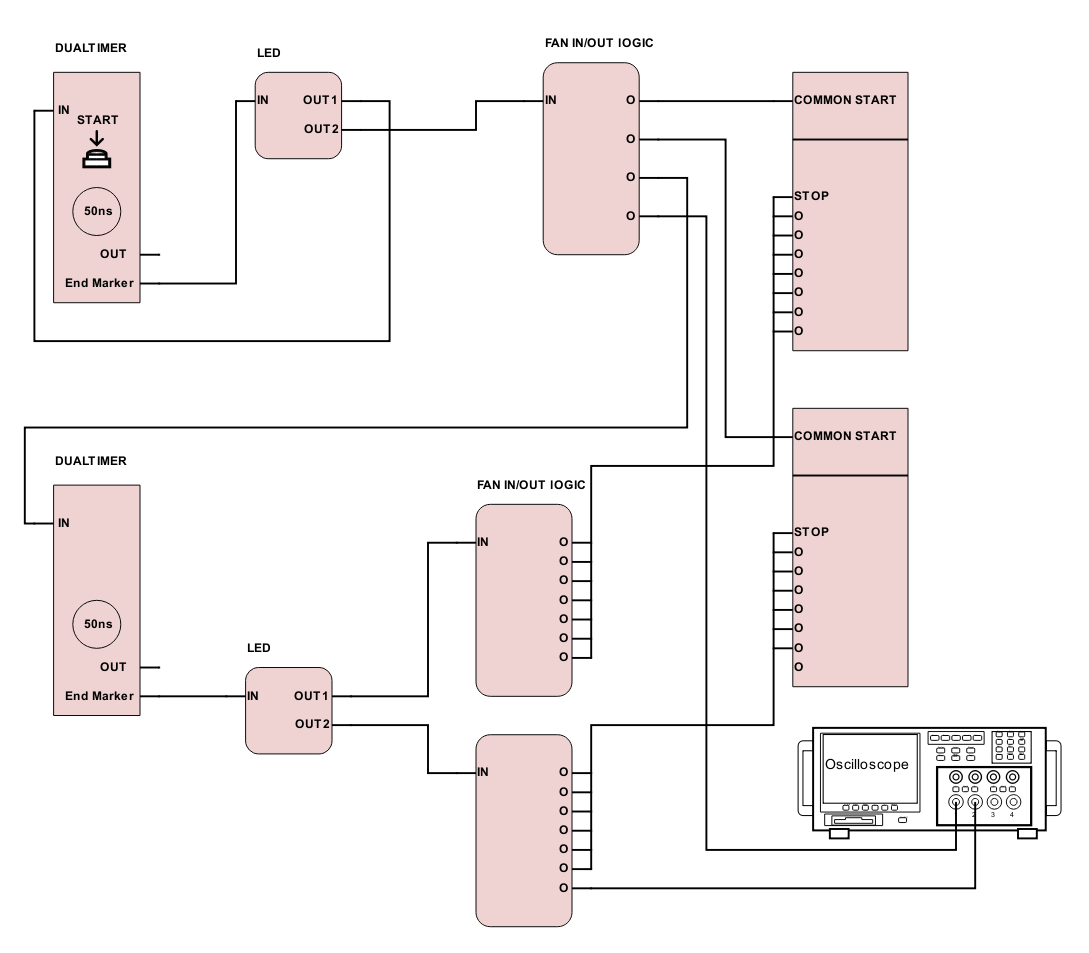
\includegraphics[width=1.\textwidth]{./SCHEMI/Calibrazione.png} % Include the image placeholder.png
		\caption{\small Schema del circuito usato per la calibrazione delle TDC}
		\label{fig:circ-calibrazione}
	\end{center}
\end{figure}
\clearpage
\section{Circuito di Acquisizione}
\label{sec:acquisizione}
Una volta selezionati gli eventi di $\mu$-stop tramite il trigger discusso in Sezione \ref{sec:trigger}, \`e necessario misurare l'intervallo di tempo trascorso
fino all'arrivo del segnale generato dall'elettrone, prodotto dal decadimento del muone.
Considerato che il tempo di vita media del muone \`e di circa 2.2 $\mu s$ \`e necessario che il circuito di acquisizione sia in grado di misurare intervalli temporali dell'ordine della decina di $\mu s$. A
tal fine sono stati utilizzati due moduli CAMAC TDC (TDC1 e TDC2) con fondoscala nominale di 5 $\mu s$ ciascuno.\\
Lo schema del circuito utilizzato per l'acquisizione \`e riportato in Figura \ref{fig:circ-acquisizione}. Il segnale proveniente dal trigger funge da common start della TDC1 e, una volta ritardato di 4.7$\mu s$ che corrisponde al valore di saturazione reale dei canali del modulo, anche della TDC2; gli stop sono invece dati da segnali provenienti dai singoli scintillatori (corrispondenti al passaggio di un $e^-$ di decadimento). Si noti che anche il segnale di common start della TDC 1 \`e in realt\`a leggermente ritardato (30 $ns$), affinch\'e i segnali formatisi sui canali P0, P1 e P2 durante un evento $\mu$-stop, arrivino sempre dopo il segnale di trigger e non producano dei falsi stop prematuri che porterebbero a una sottostima della vita media.\\
Il segnale ritardato usato come common start per la TDC2 viene inoltre sfruttato come stop per la TDC1 in modo da poter monitorare nel tempo la differenza temporale tra le due TDC e, una volta ritardato di altri 1.6 $\mu s$, come fake stop della seconda, in modo da essere sicuri che il bit LAM (look at me) del modulo venga acceso e la lettura sia effettuata.\\
Uno dei segnali proveniente dai canali di uscita del trigger viene infine ritardato di 100 $\mu s$ e utilizzato come veto. Ci\`o \`e necessario per fornire alle TDC il tempo di processare correttamente la misura di tempo. Il loro "tempo morto " \`e infatti corrispondente a circa 22 $\mu s$ ed \`e buona norma imporre un veto pari almeno al doppio.
\clearpage

\begin{figure}[H]
		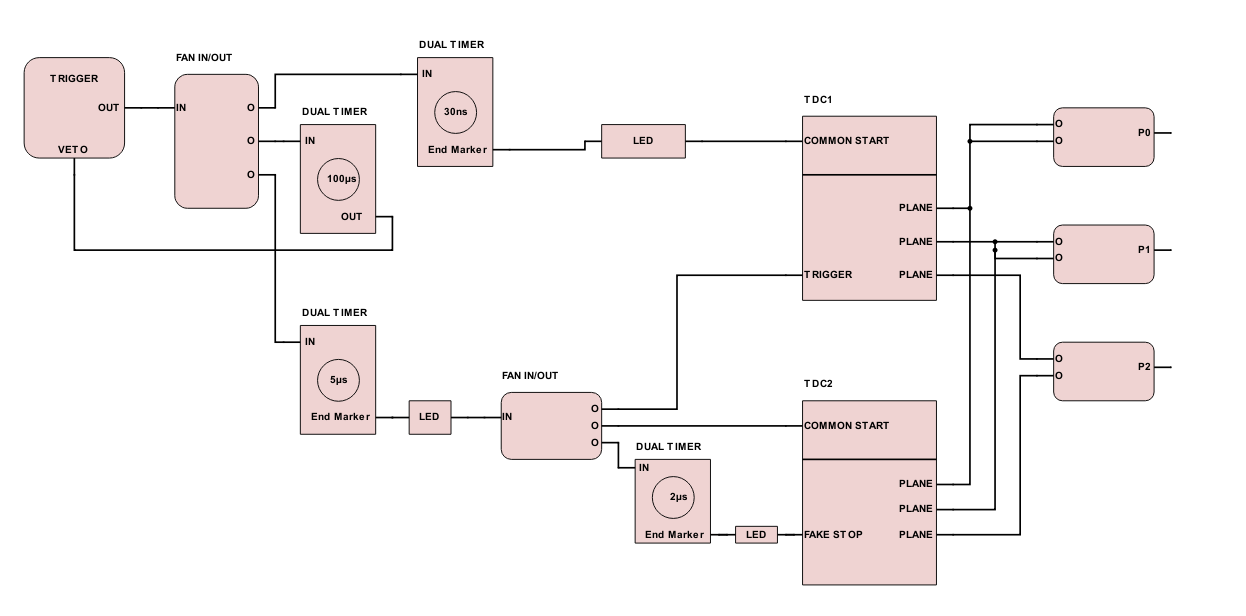
\includegraphics[width=1.2\textwidth]{./SCHEMI/FINAL.png} % Include the image placeholder.png
		\caption{\small Rappresentazione schematica del circuito usato per la misura della vita media del muone}
		\label{fig:circ-acquisizione}
	
\end{figure}

\section{Analisi Dati}
L'acquisizione dei dati si \`e svolta su un arco temporale di circa quattro giorni, per un totale di 1014917 eventi collezionati. Il processo di analisi consta principalmente dei due seguenti punti:
\begin{itemize}
  \item applicazione di tagli al fine di eliminare il fondo;
  \item fit della distribuzione dei tempi alla funzione nota, al fine di inferire la vita media del muone e altri parametri secondari dell'equazione.
\end{itemize}
Istogrammi e fit sono stati realizzati rispettivamente con le librerie MatPlotLib e SciPy di Python. \\
La funzione usata come modello per la stima dei parametri considera una legge esponenziale per il decadimento del muone e un fondo constante, dovuto al passaggio accidentale (e raro) di un secondo muone che viene scambiato per un elettrone del decadimento:
\begin{equation}
  f(t;\tau_{\mu},N_{sig},N_{bkg}) = N_{sig} \cdot \exp{(-t / \tau_{\mu})} + N_{bkg}
  \label{eqn:simple_expo}
\end{equation}
I tagli utilizzati sono stati i seguenti:
\begin{enumerate}[label=(\alph*)]
  \item eventi provenienti dal piano 1 in coincidienza con il piano 0, escludendo le coincidenze con il piano 2; con questo taglio s'intende conteggiare gli elettroni che dal ferro risalgono, passando per i piani 1 e 0;
  \item eventi provenienti dal piano 2, escludendo le coincidenze con i piani 0 e 1; questo taglio rappresenta gli elettroni che dal ferro scendono passando per il piano 2;
  \item unione dei due tagli precedenti, cos\`i da conteggiare tutti gli elettroni emessi;
  \item stesso taglio del punto precedente, ma con in pi\`u la condizione che il segnale sul piano 1 sia antecedente rispetto a quello sul piano 0, cos\`i da scartare muoni che potrebbero essere scambiati per elettroni di decadimento.
\end{enumerate}

\begin{table}[!hbt]
  \centering
  \begin{tabular}{c|c}
    \hline
    \hline
    taglio & $\tau_{\mu}$ ($\mu$s) \\
    \hline
    \hline
    a & $2.160 \pm 0.363$ \\
    b & $2.130 \pm 0.286$ \\
    c & $2.154 \pm 0.209$ \\
    d & $2.123 \pm 0.291$ \\
    \hline
    \hline
  \end{tabular}
  \caption{Risultati del fit.}
  \label{tab:res_fit}
\end{table}

In tutti e quattro i casi il fit � stato eseguito su eventi rivelati a tempi maggiori di 0.9 $\mu$s dallo START del trigger, cos� da escludere i decadimenti dei muoni negativi, caratterizzati da una vita media di circa 200 ns, che veranno considerati nella sezione successiva. Le curve dei fit, sovrapposte alle distribuzioni dei tempi, sono riportate in Fig. \ref{fig:taglioa}, \ref{fig:tagliob}, \ref{fig:taglioc} e \ref{fig:taglioa}. In Tab. \ref{tab:res_fit} sono invece riportati i valori trovati per la vita media del muone ($\tau_{\mu}$) in ogni taglio.


\begin{figure}[H]
  \centering
  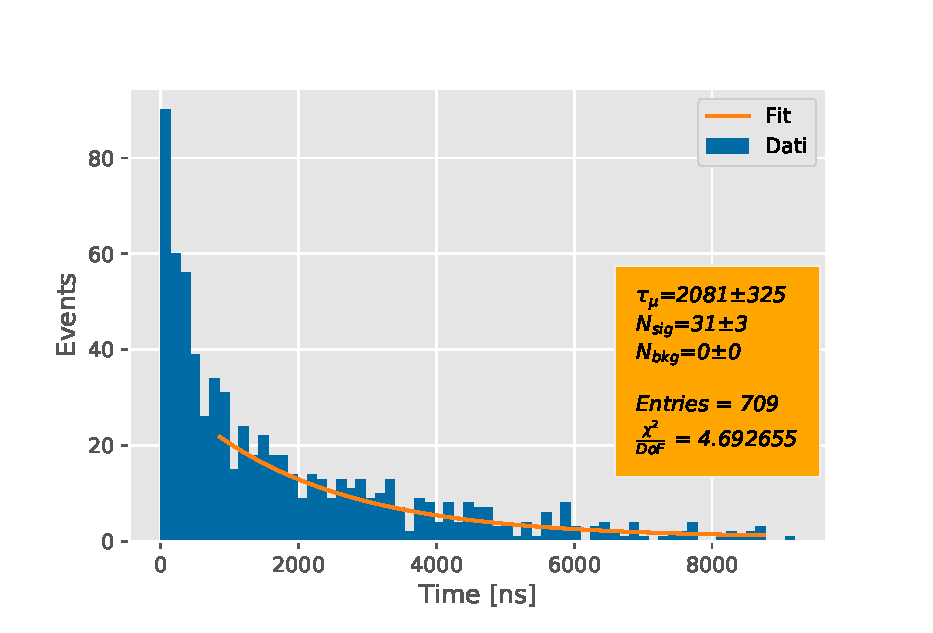
\includegraphics[width=\textwidth]{plots/piano0&1.eps}
  \caption{Taglio (a)}
  \label{fig:taglioa}
\end{figure}

\begin{figure}[H]
  \centering
  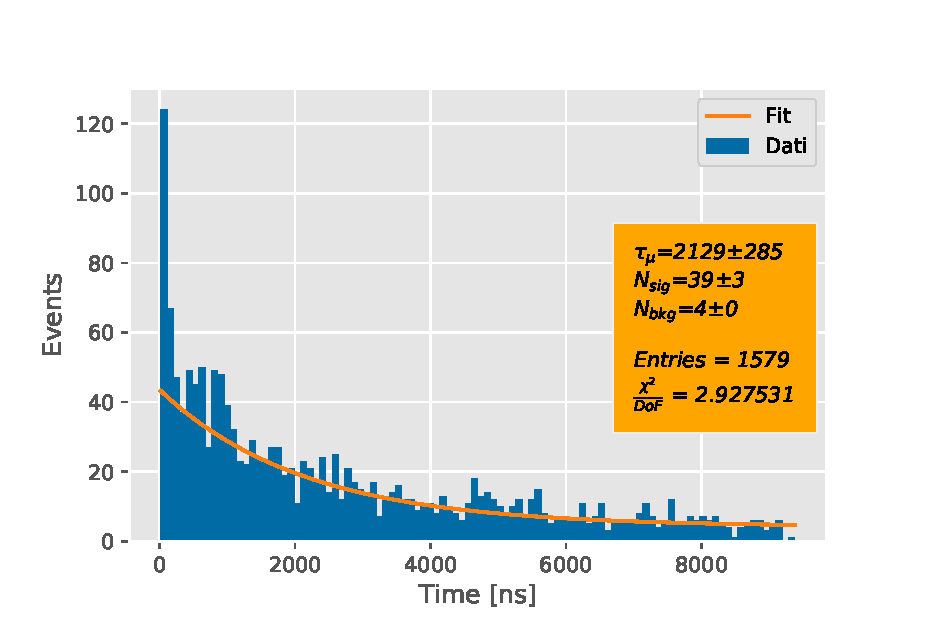
\includegraphics[width=\textwidth]{plots/piano2.eps}
  \caption{Taglio (b)}
  \label{fig:tagliob}
\end{figure}

\begin{figure}[H]
  \centering
  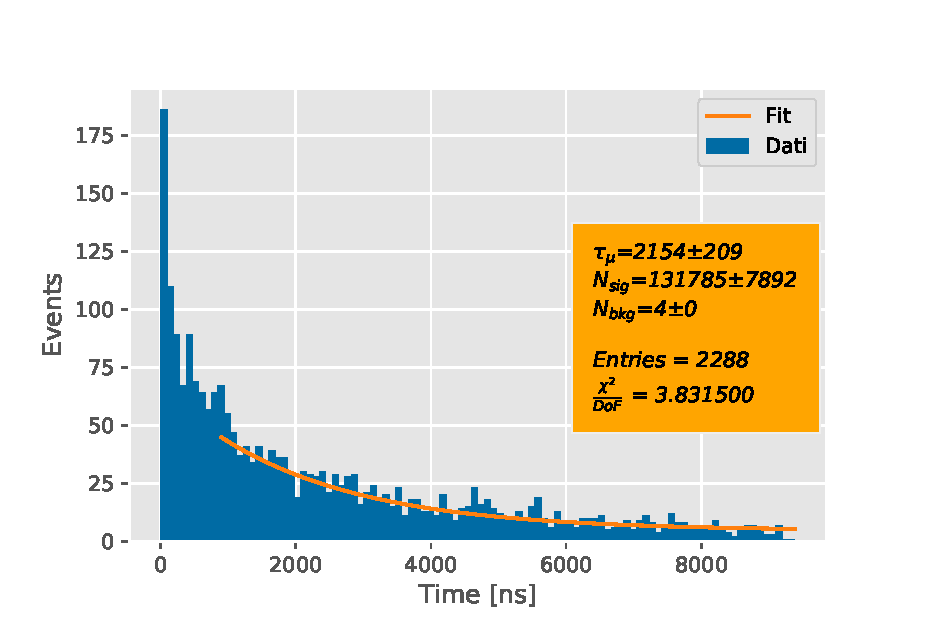
\includegraphics[width=\textwidth]{plots/soft_nopiano1.eps}
  \caption{Taglio (c)}
  \label{fig:taglioc}
\end{figure}

\begin{figure}[H]
  \centering
  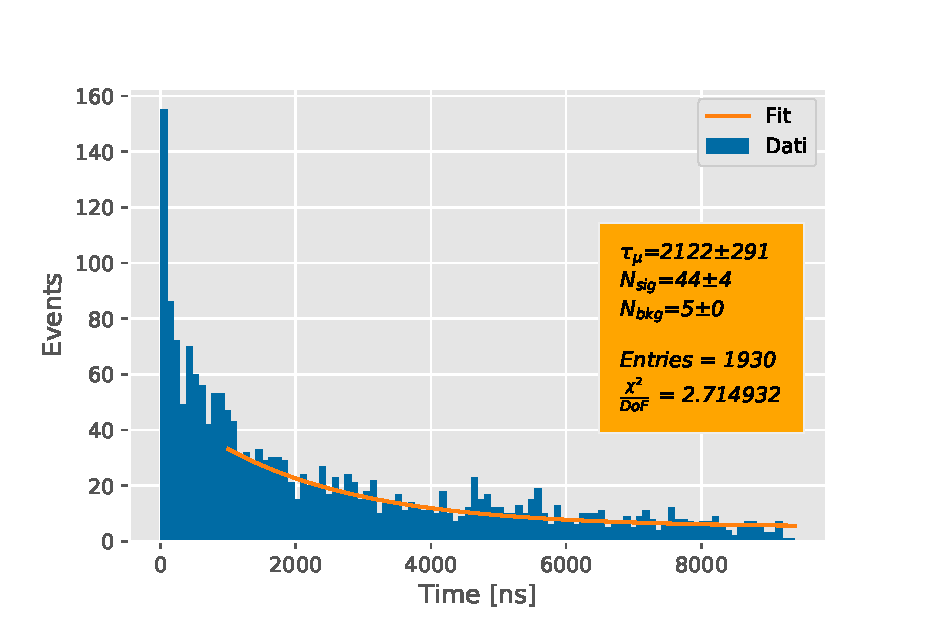
\includegraphics[width=\textwidth]{plots/hard_nopiano1.eps}
  \caption{Taglio (d)}
  \label{fig:tagliod}
\end{figure}


\subsection{Cattura dei muoni negativi.}
Ci si propone ora di stimare un effetto implicitamente trascurato nelle sezioni precedenti, ovvero che la vita media dei muoni negativi nella materia differisce dalla stessa quantit\`a misurata nel vuoto. Il motivo \`e l'interazione elettromagnetica tra i $\mu^{-}$ e i nuclei atomici.
\paragraph{Cattura muonica}
Quando entrano in un materiale, i $\mu^{-}$ vengono rallentati e formano atomi muonici, ovvero atomi nei quali un elettrone \`e rimpiazzato da un muone negativo. Una volta formato l'atomo muonico, il $\mu^{-}$ pu\`o decadere come nel vuoto oppure essere catturato dal nucleo, con conseguente emissione di neutroni o particelle cariche.

La vita media del muone negativo in un atomo muonico \`e dunque determinata da questi due processi concorrenti. Detti $\tau^{-}_{decay}$ la vita media del $\mu^{-}$ nel vuoto e $\tau^{-}_{capture}$ quella nella cattura neutronica, \`e possibile scrivere la vita media totale come:
\begin{equation}
  \frac{1}{\tau_{A}} = \frac{1}{\tau^{-}_{decay}} + \frac{1}{\tau^{-}_{capture}}
  \label{eqn:neg_muon_total}
\end{equation}

Essa, nella sua componente dovuta alla cattura, dipende fortemente dal numero atomico $Z$ del materiale. Nel caso del ferro ($Z=26$) si hanno:
\begin{equation}
  \tau^{-}_{capture}=0.22\, \mu\text{s}
  \label{eqn:tau_cap_iron}
\end{equation}

\begin{equation}
  \tau_{A}=0.20\, \mu\text{s}
  \label{eqn:tau_tot_iron}
\end{equation}
Si sottolinea che negli esperimenti \`e sempre la $\tau_{A}$ ad essere misurata.

\paragraph{Misura e risultati.}
In fase di analisi dati, \`e possibile tenere conto del diverso contributo dei $\mu^{-}$ inserendo nel modello un ulteriore termine esponenziale. Si avr\`a:

\begin{equation}
  f(t;\tau_{\mu},\tau_{A},N_{sig},N_{A},N_{bkg}) = N_{sig}\exp{(-t/\tau_{\mu})} + N_{A}\exp{(-t/\tau_{A})} + N_{bkg}
  \label{eqn:complex_expo}
\end{equation}

Il taglio imposto \`e stato lo stesso del punto (c) del paragrafo precedente. Sono stati eseguiti due tipi di fit: nel primo sia $\tau_{\mu}$ che $\tau_{A}$ sono liberi, mentre nel secondo si \`e fissato $\tau_{\mu}=2.197\, \mu$s come riportato in \cite{pdg}. I valori stimati per $\tau_{A}$ e $\tau^{-}_{capture}$, dove quest'ultimo \`e trovato applicando (\ref{eqn:neg_muon_total}), sono riportati in Tabella \ref{tab:negative_muon}. Istogrammi e plot sono invece riportati in Fig. (\ref{fig:soft_doubleexp}) e (\ref{fig:soft_doubleexp_fixed}).

\begin{table}[H]
  \centering
  \begin{tabular}{c|c|c|c}
    \hline
    \hline
    Fit & $\tau_{\mu}$ ($\mu$s) & $\tau_{A}$ ($\mu$s) & $\tau^{-}_{capture}$ ($\mu$s) \\
    \hline
    \hline
    $\tau_{\mu}$ libero & $2.130 \pm 0.375$ & $0.327 \pm 0.094$ & $0.386 \pm 0.071$\\
    $\tau_{\mu}$ fissato & & $0.333 \pm 0.061$ & $0.393 \pm 0.011$ \\
    \hline
    \hline
  \end{tabular}
  \caption{Valori ottenuti fittando i dati ad un modello che considera anche la vita media dei muoni negativi. Si pu\`o vedere che i valori di $\tau_{A}$ e $\tau_{capture}^{-}$ si discostano leggermente dai valori attesi, anche considerando le incertezze sperimentali. Per quanto riguarda invece $\tau_{\mu}$, esso risulta compatibile con il valore atteso entro l'incertezza.}
  \label{tab:negative_muon}
\end{table}

\begin{figure}[H]
  \centering
  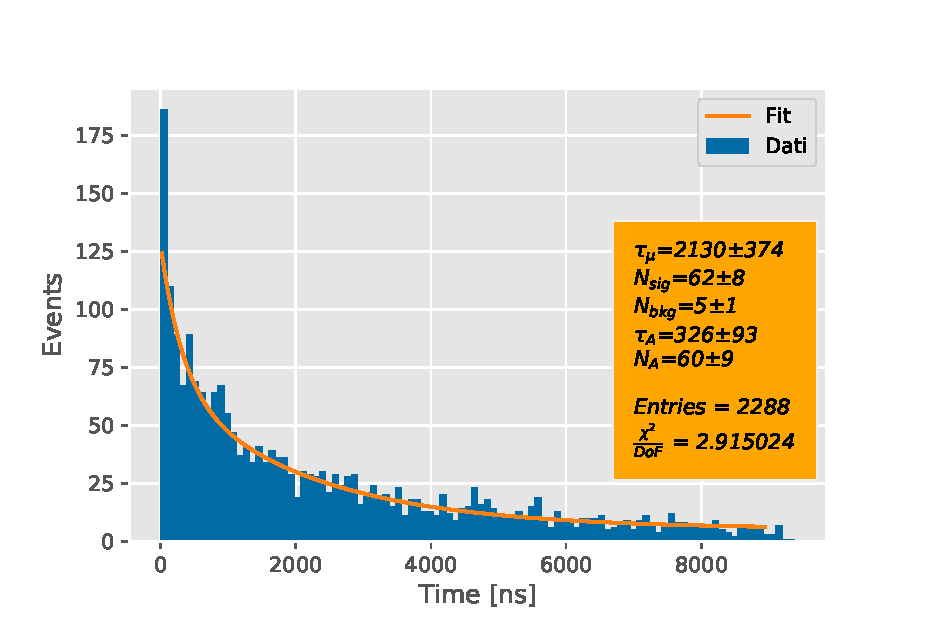
\includegraphics[width=\textwidth]{plots/soft_doubleexp.eps}
  \caption{Taglio (c) con fit ad un modello che comprende due termini esponenziali; sia $\tau_{\mu}$ che $\tau_{A}$ sono liberi.}
  \label{fig:soft_doubleexp}
\end{figure}

\begin{figure}[H]
  \centering
  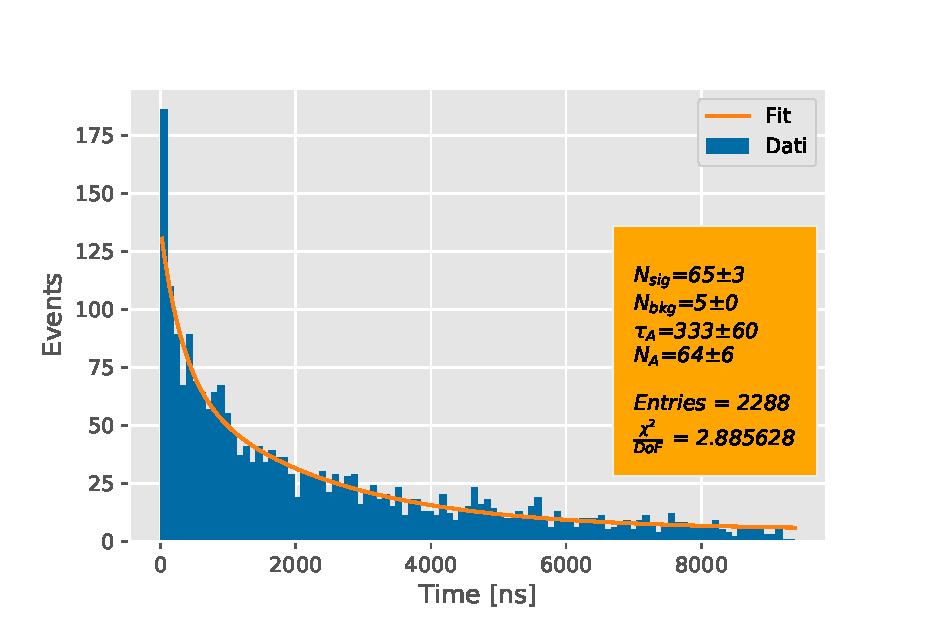
\includegraphics[width=\textwidth]{plots/soft_doubleexp_fixed.eps}
  \caption{Taglio (c) con fit ad un modello che comprende due termini esponenziali; $\tau_{\mu}$ \`e fissato, mentre $\tau_{A}$ � libero.}
  \label{fig:soft_doubleexp_fixed}
\end{figure}

Poich\`e l'errore relativo su $\tau_{A}$ resta comunque piuttosto alto ($\approx 30 \%$ nel caso di due parametri liberi, $\approx 20 \%$ nel caso di uno), non includeremo questi risultati nelle conclusioni, attribuendo a quest'ultimo studio lo scopo di giustificare la decisione di escludere gli eventi a tempi molto brevi dell'analisi precedente.

%%%%%%%%%%%%%%%%%%%%%%%%%%%%%%%%%%%%%%%%%per fare le conclusioni
\chapter{Conclusioni}
%\addcontentsline{toc}{chapter}{Conclusioni}

Il procedimento di misura della vita media del muone pu\`o riassumersi in due parti principali:
\begin{itemize}
  \item nella prima si \`e configurato l'apparato sperimentale: \`e stato realizzato il circuito di trigger per la determinazione degli eventi di $\mu$-stop, sono state individuate le tensioni di discriminazione, valutati i ritardi sui segnali e infine calibrati i TDC;
  \item nella seconda sono stati raccolti e analizzati i dati: l'analisi \`e stata effettuata determinando i tagli opportuni da applicare agli eventi raccolti negli istogrammi.
\end{itemize}
Si sceglie di utilizzare come miglior stima quella ottenuta dal taglio (c) descritto nella sezione precedente, essendo quello fisicamente pi\`u corretto. Il risultato finale ottenuto \`e quindi di
\begin{equation}
  \tau_{\mu} = 2.123 \pm 0.291 \mu\text{s}
  \label{final_res}
\end{equation}
consistente con quello riportato in letteratura \cite{pdg}.

\end{document}
